%%\title{Global Reference System}
%  Changed by: Chris ISELIN, 17-Jul-1997 
%  Changed by: Hans Grote, 10-Jun-2002 

\section{Global Reference System}

The \hyperlink{global}{global reference orbit} of the accelerator is
uniquely defined by the sequence of physical elements. The local
reference system (\textit{x}, \textit{y}, \textit{s}) may thus be
referred to a global Cartesian coordinate system (\textit{X},
\textit{Y}, \textit{Z}) (see \hyperlink{global}{Figure 1}). The
positions between beam elements are numbered 0,...,i,...n. The local
reference system  (\textit{x$_i$, y$_i$, s$_i$}) at position \textit{i},
i.e. the displacement and direction of the reference orbit with respect
to the system (\textit{X}, \textit{Y}, \textit{Z}) are defined by three
displacements  (\textit{X$_i$}, \textit{Y$_i$}, \textit{Z$_i$}) and
three angles (\textit{Theta$_i$}, \textit{Phi$_i$}, \textit{Psi$_i$})

The above quantities are defined more precisely as follows:  
\begin{itemize}
   \item X: Displacement of the local origin in \textit{X}-direction. 
   \item Y: Displacement of the local origin in \textit{Y}-direction. 
   \item Z: Displacement of the local origin in \textit{Z}-direction. 
   \item \href{theta}{THETA}: Angle of rotation (azimuth) about the
     global \textit{Y}-axis, between the global \textit{Z}-axis and the
     projection of the reference orbit onto the (\textit{Z},
     \textit{X})-plane. A positive angle THETA forms a right-hand screw
     with the \textit{Y}-axis. 
   \item \href{phi}{PHI}: Elevation angle, i.e. the angle between the
     reference orbit and its projection onto the (\textit{Z},
     \textit{X})-plane. A positive angle PHI correspond to increasing
     \textit{Y}. If only horizontal bends are present, the reference
     orbit remains in the (\textit{Z}, \textit{X})-plane. In this case
     PHI is always zero. 
   \item \href{psi}{PSI}: Roll angle about the local \textit{s}-axis,
     i.e. the angle between the intersection (\textit{x}, \textit{y})-
     and (\textit{Z}, \textit{X})-planes and the local
     \textit{x}-axis. A positive angle PSI forms a right-hand screw with
     the \textit{s}-axis. 
\end{itemize} 

The angles (THETA, PHI, PSI) are \textbf{not} the Euler angles. The
reference orbit starts at the origin and points by default in the
direction of the positive \textit{Z}-axis. The initial local axes
(\textit{x}, \textit{y}, \textit{s})  coincide with the global axes
(\textit{X}, \textit{Y}, \textit{Z}) in this order. The six quantities
(X$_0$, Y$_0$, Z$_0$, THETA$_0$, PHI$_0$, PSI$_0$) thus all have zero
initial values by default. The program user may however specify
different initial conditions.  

Internally the displacement is described by a vector \textit{V} and the
orientation by a unitary matrix \textit{W}. The column vectors of
\textit{W} are the unit vectors spanning  the local coordinate axes in
the order (\textit{x, y, s}). \textit{V} and \textit{W} have the values:  


%%\includegraphics{null}
%VW
\[
V =
 \begin{pmatrix}
  X \\
  Y \\
  Z
 \end{pmatrix}
, \quad\quad
W=\Theta\Phi\Psi
\]

 where 

%%\includegraphics{null}
%PhiThetaPsi
\[
\Theta =
 \begin{pmatrix}
  \cos \theta  & 0 &  \sin \theta \\
  0            & 1 &  0 \\
  -\sin \theta & 0 &  \cos \theta
 \end{pmatrix}
, \quad
\Phi =
 \begin{pmatrix}
  1 & 0          &  0 \\
  0 & \cos \phi  &  \sin \phi \\
  0 & -\sin \phi &  \cos \phi
 \end{pmatrix}
, \quad
\Psi =
 \begin{pmatrix}
  \cos \psi &  -\sin \psi & 0 \\
  \sin \psi &  \cos \psi  & 0 \\
  0	    &	0	  & 1 
 \end{pmatrix}
.
\]

The reference orbit should be closed and it should not be twisted. This
means that the displacement of the local reference system must be
periodic with the revolution frequency of the accelerator, while the
position angles must be periodic modulo(2 pi) with the revolution
frequency. If PSI is not periodic module(2 pi), coupling effects are
introduced. When advancing through a beam element, MAD computes
\textit{V$_i$} and \textit{W$_i$} by the recurrence relations  

\textit{V$_i$ = W$_i-1$R$_i$ + V$_i-1$}, \textit{W$_i$ = w$_i-1$S$_i$}. 

The vector \textit{R$_i$} is the displacement and the matrix
\textit{S$_i$} is the rotation of the local reference system  at the
exit of the element \textit{i} with respect to the entrance  of the same
element. The values of \textit{R$_i$} and \textit{S$_i$} are listed in
the:   \href{local_system.html#straight}{straight reference system} for
each physical element type.  
%%%\begin{center}
%\href{global}{
%%%\includegraphics{null}}
%
%\textbf{Figure 1:} Global Reference System 
%%%\end{center}
\begin{figure}[h!]
  \centering
	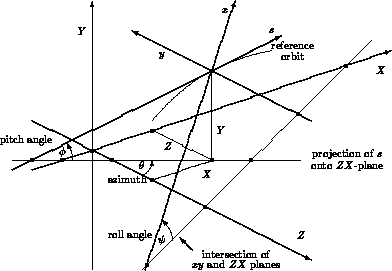
\includegraphics{figures/global.png}
  \caption{\href{global}{Global Reference System }}%{\textbf{Figure 1:} Local Reference System}}
\end{figure}

%\href{http://www.cern.ch/Hans.Grote/hansg_sign.html}{hansg}, January 24, 1997 

